\section{Introduction}
\label{sec:intro}
Frontier models are rented, not downloaded.  You send a request to an API and an answer
comes back.  The weights stay hidden.  But the API is not a blank wall.  Every answer is
produced by a real pipeline: a tokenizer, an embedding table, a stack of attention or
state-space blocks, an output projection, and a serving system wrapped around all of
it.  Each of these stages leaves small traces in what comes back: the token counts on
the bill, the score vectors (logprobs), the timing, and the way errors are reported.
This paper asks one quantitative question and answers it with a measurement:
\begin{quote}
\textbf{What can an API reveal about a hidden computational system?  Exactly how much of
its functional architecture can be identified, and where does identification provably
stop?}
\end{quote}

The answer is not a yes or a no.  It is a \emph{four-way boundary}.  Some properties
are \textbf{identified} outright by sending controlled requests.  Some are
\textbf{cost-limited}: they can be separated in principle, but each request buys only a
little evidence, so the real question is how many requests the job needs.  We answer
that with an estimate of the information one request carries, written $\hat\kappa$,
under a stated family of probes.  Some are \textbf{access-limited}: the API does not
expose the channel at all.  Top-5-only logprobs, buffered streams, and a deployment cap
are all examples.  And some are \textbf{non-identifiable}: two different architectures
provably produce identical observations, and we show the pair explicitly.  In formal
terms, what we recover is the \emph{equivalence class} $[\omega]_{\mathcal C,\mathcal
X}$, the set of all configurations that would look identical through the channels we
have, and, for each property $g$, the \emph{identified set} $\mathcal
I_g(\omega;\mathcal C,\mathcal X)$, the values of that property that remain possible.
We never recover the literal configuration $\omega$, and we do not pretend to.

\begin{figure}[t]\centering
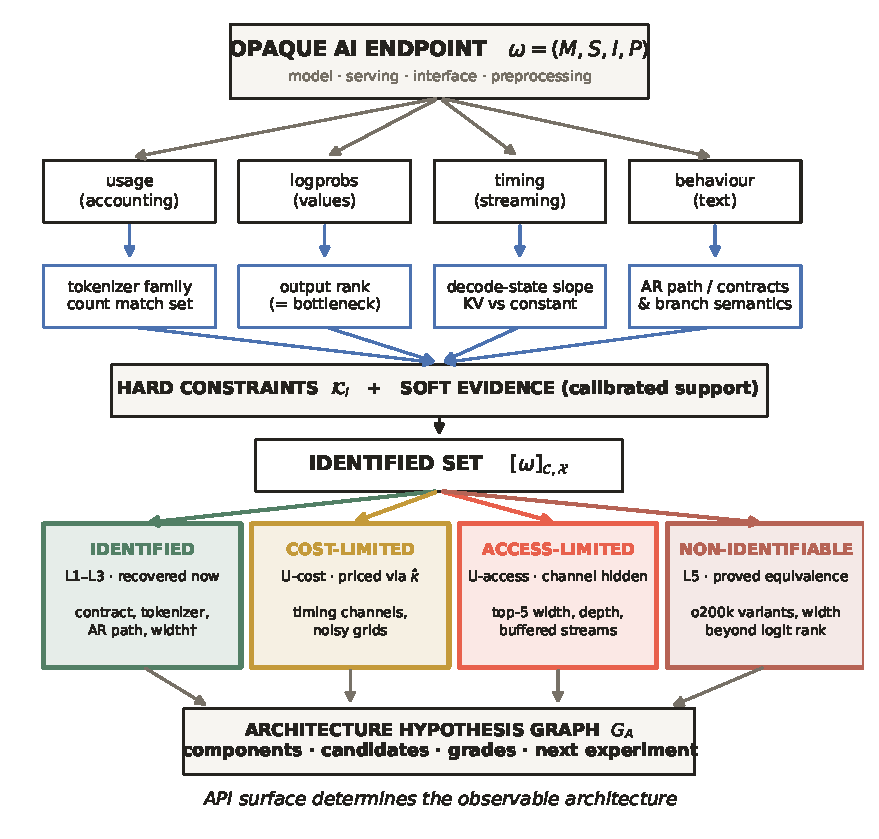
\includegraphics[width=.8\textwidth]{figures/fig_v4_masterflow.pdf}
\caption{The whole paper on one page.  An opaque endpoint $\omega=(M,S,I,P)$ is probed
through four kinds of channel: usage accounting, logprobs, timing, and behaviour.
Each observation becomes either a hard constraint or a piece of graded soft evidence.
Together they define the identified set $[\omega]_{\mathcal C,\mathcal X}$, which sorts
every component into one of four classes: identified, cost-limited, access-limited, or
witnessed non-identifiable.  What remains is the architecture hypothesis graph $G_A$: an
honest reconstruction, with a grade and a named next experiment attached to every
node.}
\label{fig:masterflow}
\end{figure}

\begin{table}[t]\centering\small
\caption{The identification boundary, measured.  Left: the functional components the
battery identifies, with accuracy measured on \benchname{} (known models served behind an
anonymous API, with detector thresholds frozen in advance).  Right: the components that
stay open, each with the reason.  The reason is always one of three things: a proved
equivalence witness (grade L5), a channel whose per-request information $\kappa$ we have
estimated, or a named next experiment.  Production rows are graded by how reliable the
detector proved on the benchmark, never simply asserted.}
\label{tab:boundary}
\begin{tabularx}{\textwidth}{@{}Y c Y@{}}
\toprule
\textbf{Identified (with measured accuracy)} & \textbf{Bench} & \textbf{Open, and why}\\
\midrule
API contract and serving limits & \ContractAcc & depth: compute and queueing are tangled
together; identity-layer witness (App.~A)\\
Tokenizer count-family \& template overhead & \TokenizerAcc & exact vocabulary: the
reference set has gaps (DeepSeek: 465 unresolved entries)\\
AR-compatible generation contract vs encoder readout & \FamilyPathAcc & ---\\
Transformer vs constant-state (SSM) split & \SsmSplitAcc & production span limit: decode
growth is drowned in noise at $\le$12k context (U-cost)\\
Output bottleneck width $d$ (rich access) & \GeomResolvedAcc & top-5-only access: rank
$\le$ a handful of columns (witness, Prop.~\ref{prop:rank})\\
Wire numeric grid (fp32/bf16/fp16) & \DtypeAcc & internal compute dtype: transport rounding
hides it\\
Dense vs MoE feed-forward & \MoeAcc & weakest detector; production claims discounted
to match (Sec.~\ref{sec:production})\\
Decision branch/readout structure (JEV) & $p=\JevPermP$ & physical prefill sharing:
only the operator can attest it\\
\bottomrule
\end{tabularx}
\end{table}

\paragraph{Why a benchmark changes the claims.}
Earlier black-box architecture work reports demonstrations on subjects the authors chose
themselves.  We did something different.  We took \BenchN{} known checkpoints, covering
dense transformers, Mamba SSMs, mixture-of-experts models (including OLMoE-1B-7B), an MLA
mechanics subject, masked encoders, and an encoder-decoder, plus variants that change
only the number format, the batching, or the routing.  We served all of them behind one
API contract whose capabilities match a real production API.  We froze the protocol and
every detector threshold.  Only then did we measure what the scanner gets right.  The
\BenchN{} subjects are built on \BenchArchs{} distinct base checkpoints; the rest are
serving variants of the GPT-2 checkpoint (precision, quantisation, wire rounding,
batching) plus a two-checkpoint router.  So every accuracy interval in this paper is
bootstrapped at the checkpoint level.  Variants of one model are never counted as
independent architectures.

Three results reshaped the paper.  (i) The flagship ``decoder-only 0.97'' score from our
own earlier version did not separate transformers from state-space models at all.  Both
are autoregressive decoders, so both pass that test.  We built and validated a
decode-state probe that does separate them (Sec.~\ref{sec:howfar}).  (ii) Output-width
recovery is exact up to the widest model we tested, as long as the probe uses more prompt
rows than the model has width.  Under top-5-only access it is empty.  We prove why and
then demonstrate it (Prop.~\ref{prop:rank}).  (iii) The domain-timing MoE detector is
genuinely weak (accuracy \MoeAcc), so every production MoE claim is reported at that
reliability.

\paragraph{Production case studies.}
We then point the battery at three live endpoints: GPT-4o-mini, DeepSeek-V3.2, and the
JEV decision model.  On each it reconstructs the input/output boundary, the tokenizer
count-family, the autoregressive generation path, the numeric format on the wire, and the
serving behaviours.  Every claim imports its reliability from the benchmark.  DeepSeek's
MoE lean agrees with its published design.  Its prefill time on fresh prompts grows more
slowly than quadratically (exponent \DsFreshExp, 95\% CI \DsFreshCI, $n=\DsFreshN$).
That is compatible with its documented sparse attention, but it does not single it out,
and our same-hardware control shows exactly why (Sec.~\ref{sec:attncontrol}).

\paragraph{The evidence hierarchy.}  The paper's strength runs from the top down.
Tier 1 is the formal non-identifiability witnesses.  These are mathematically clean.
Tier 2 is detector validation against known ground truth on \benchname{}.  Here the
instrument is measured, not merely plausible.  Tier 3 is the controlled causal probes:
transformer versus SSM, JEV branch isolation, deliberate serving changes, and
same-hardware timing controls.  Tier 4 is the interpretation of the three production
systems.  \textbf{The benchmark and the boundary are the contribution; the production
systems are demonstrations.}  They are graded demonstrations, because their detectors
were measured first.

\paragraph{Contributions.}
\begin{enumerate}[label=\textbf{C\arabic*.},leftmargin=2.6em]
\item A clean statement of the problem: black-box architecture work is \emph{functional
  architecture identification under API observability constraints}.  This brings
  three tools: the equivalence class $[\omega]_{\mathcal C,\mathcal X}$, the Forensic
  Layer Model (model $\neq$ serving $\neq$ interface $\neq$ preprocessing), and the
  four-way boundary.  It also includes a channel-closure study showing that how much of
  an architecture is observable is itself a choice the API designer makes
  (Sec.~\ref{sec:observability}).
\item \benchname{}, a blind ground-truth benchmark: \BenchN{} served subjects, one
  anonymous contract, a frozen protocol, commit-reveal blind fixtures, and every journal
  released.
\item An evidence-ranking instrument that has been tested, not just described: evidence
  combination that respects dependence between probes, with measured calibration; a
  validated decode-state probe that separates transformers from SSMs; and width recovery
  with a measured coverage curve.
\item Identifiability made practical: two scoped witnesses (one built for real, with zero
  observable difference), plus a query-cost bound with per-channel $\hat\kappa$
  estimates, offered as a secondary and explicitly conditional tool
  (Sec.~\ref{sec:kappa}).
\item Baselines (NightVision-style and LLMmap-style, run on the same subjects) and a live
  planner study.  The planner study produced a negative result, and we report it: a
  simple static ordering is not beaten by our information-gain planner.
\end{enumerate}

\paragraph{Scope.} All probing used configured, authorised accounts with bounded
budgets.  We accessed no weights, no training data, and no private tenants.  Dual-use
considerations and release status are in Sec.~\ref{sec:ethics}.
